\documentclass[9pt]{IEEEtran}

\usepackage[english]{babel}
\usepackage{subcaption}
\usepackage{graphicx}
\usepackage{epstopdf}
\usepackage{fancyhdr}
\usepackage{amsmath}
\usepackage{amsthm}
\usepackage{amssymb}
\usepackage{url}
\usepackage{array}
\usepackage{textcomp}
\usepackage{listings}
\usepackage{hyperref}
\usepackage{xcolor}
\usepackage{colortbl}
\usepackage{float}
\usepackage{gensymb}
\usepackage{longtable}
\usepackage{supertabular}
\usepackage{multicol}
\usepackage{booktabs}

\usepackage[utf8x]{inputenc}

\usepackage[T1]{fontenc}
\usepackage{lmodern}
\input{glyphtounicode}
\pdfgentounicode=1

\graphicspath{{./figures/}}
\DeclareGraphicsExtensions{.pdf,.png,.jpg,.eps}

% correct bad hyphenation here
\hyphenation{op-tical net-works semi-conduc-tor trig-gs}

% ============================================================================================

\title{\vspace{0ex}
Project 4: Advanced Tracking}

\author{Katarina Brešar\vspace{-4.0ex}}

% ============================================================================================

\begin{document}

\maketitle

\section{Introduction}

In this assignment, we tested how motion models combined with the Kalman filter can be used to predict the future position of an object.
We tested three different models: Random Walk, Nearly Constant Velocity and Nearly Constant Acceleration and
analyzed how the parameters of the Kalman filter affect the performance of the tracking. We also
implemented a Particle filter tracker and analyzed how different parameters of the tracker affect the performance. 
We tested our implementation on the VOT2014 dataset and analyzed the results in terms of average overlap,
number of failures and tracking speed. 

\section{Experiments}

\subsection{Motion Models and Kalman Filters}

We first ran the Kalman filter method on a spiral curve using RW, NCV and NCA motion models. The matrices that we used
are in the appendix section.
Using different values of parameters $q$ and $r$ we observed how the filters performance changed. In figure~\ref{fig:kalman:diff_params} we
can see the effect of setting $q = [1,5,100]$ and $r = [1,5,100]$. We're interested in the relationship between these two parameters.
When they are both small the filter is trusting both the model and the measurments.
Setting $q$ to $100$  (and leaving $r$ small) meant that the motion model is highly uncertain, so the object 
might deviate a lot from the predicted path. 
So the filter trusts the measurments almost entirely (as we can see in the figure). Setting $q$ to a 
smaller value the filter will trust the motion model more so the trajectory is smoother,
but it doesn't follow the measurments as closely. Setting $r$ to a smaller value means
that the measurments are more accurate, so the filter will trust them more. Like in the figure where $q$ was large
and $r$ was small for all three models.
The RW model is especially sensitive as it lacks momentum, it relies completely on measurments to follow the curve. We can see how the filter
is lagging behind the measurments at sharp turn as it assumes the object is static. The NCV model is better at following the spiral, because
it also tracks velocity. Whereas the NCA model overshot the curve at tight corners because it also tracks acceleration, which becomes
a problem when the curves radius changed quickly.



\begin{figure}[h!]
    \centering
    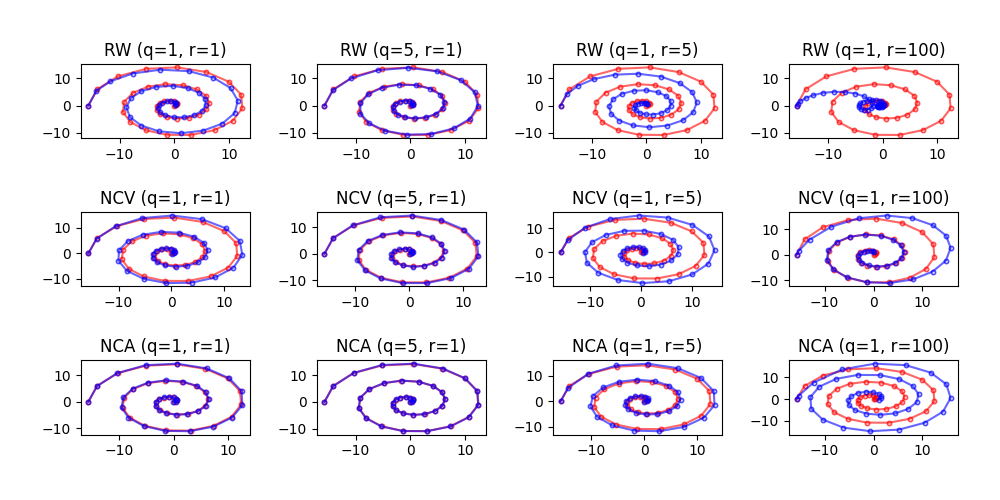
\includegraphics[width=0.5\textwidth]{Figures/kalman_diff_params.png}
    \caption{Kalman filter performance. Blue curve: filtered trajectory, Red curve: measured trajectory}
    \label{fig:kalman:diff_params}
\end{figure}

We also ran the tests on a rectangle path as seen in figure~\ref{fig:kalman:rectangle}. We can see
that all the models struggle with the 90 degree corners when $r > q$ (meaning the filter trusts the model more than the measurments)
since the assume the objects travels at a straight line. The RW is the worst at handling the corners, because it has no momentum,
the other two are better at it, but still overshoot the corners. When $q > r$, random walk
fails completely (as expected with no momentum) and NCA performs the best as it can quickly adjust to the new direction.
On the sine wave path (figure~\ref{fig:kalman:sine}) NCV model performs well, it's "faster" than the measurments since it assumes a nearly constant velocity.
NCa model performs the best, because it quikcly adjusts to the changing direction, but RW model performs worst when we're trusting the model more
than the measurments.

\begin{figure}[h!]
    \centering
    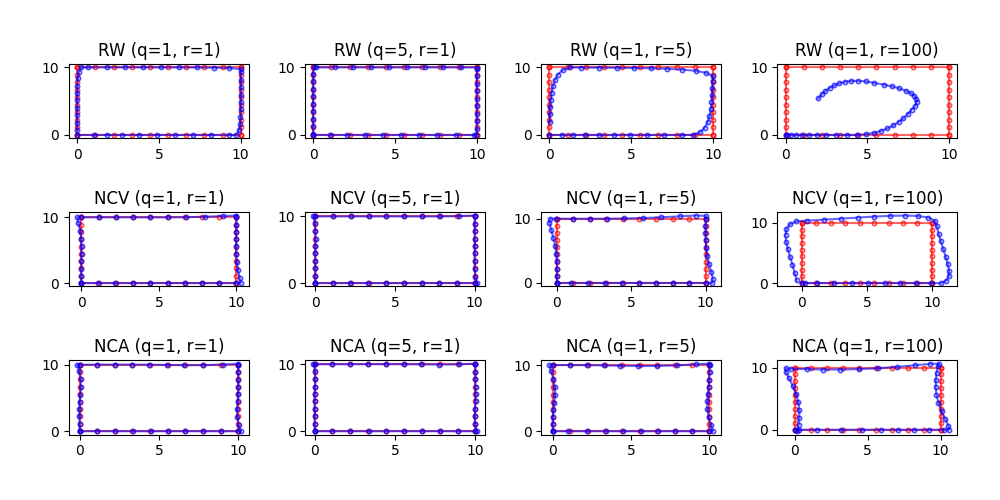
\includegraphics[width=0.4\textwidth]{Figures/kalman_rectangle.png}
    \caption{Kalman filter performance on rectangle path. Blue curve: filtered trajectory, Red curve: measured trajectory}
    \label{fig:kalman:rectangle}
\end{figure}


\begin{figure}[h!]
    \centering
    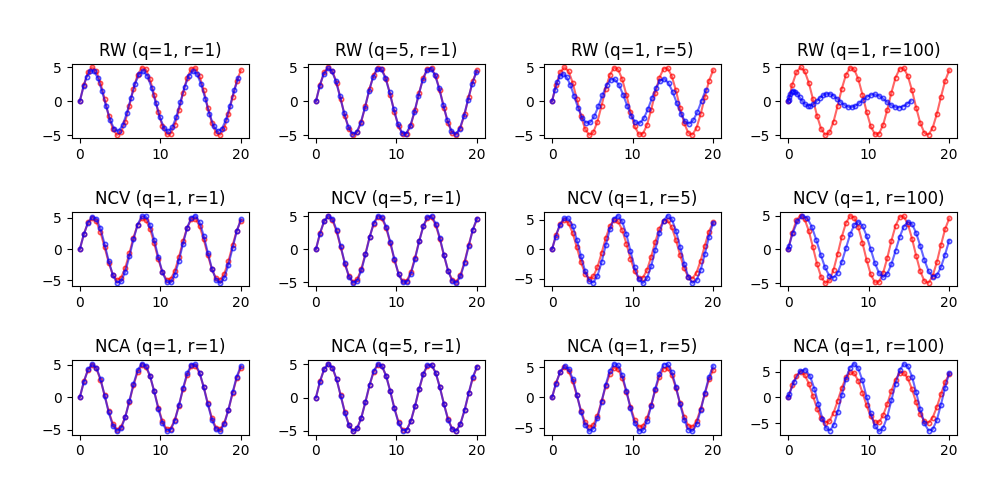
\includegraphics[width=0.4\textwidth]{Figures/kalman_sine.png}
    \caption{Kalman filter performance on sine wave path. Blue curve: filtered trajectory, Red curve: measured trajectory}
    \label{fig:kalman:sine}
\end{figure}


\subsection{Particle Filter Tracker}
We implemented the particle filter tracker using the NCV motion model and a color histogram visual model using Hellinger
distance to measure similarity between histograms. We also used na Epanechnikov kernel to give more weight
to pixels closer to the center of the target when extracting the histogram.The visual model is then updated using
a factor $\alpha$ to control how much the model should adapt to changes in the targets appearance.
We used $N$ particles to represent possible states of the 
target. We tested the tracker on the VOT2014 dataset
and got the following results: average overlap over all sequences of $0.48$, total number of failures
$55$ and average tracking speed of $41.4$ FPS. Note that for this experiment we used the following parameters:
$N = 100$ particles, $q = 0.1 * ||\text{target size}||$, color histogram with $16$ bins,
epanechnikov kernel for histogram extraction and $\alpha = 0.05$ for visual model update. We noticed that NCV provided a robust prior for standard objects, but the color histogram was sensitive to 
rapid scale changes and illumintation shift, which lead to failures in some sequences.

\subsubsection{Number of particles}
The number of particles $N$ is critical for speed of the tracker, as each particle requires histogram extraction
and weight calculation. We tested $5$ sequences with $N = [200,100,50,25]$ and got the results seen in 
table~\ref{tab:particle:N_diff}. Descreasing the number of particles significantly increased the speed of the tracking. This
makes sense since less particles means less histogram extractions and weight calculations. However, the average overlap
and failures did not change significantly. It seems that the optimal number of particles is $100$ since it provided
a good balance between accuracy, robustness and speed. Interestingly when $N=200$ the number of failures was $60$, when
we'd expect it to be lower. But this could be due to randomness. Maybe it was just "stochastically unlucky" and the
particles were not well distributed in some frames, causing the tracker to lose the target. Or maybe
the higher number of particles caused the tracker to be more sensitive to noise in the histogram, which could lead to further failures.

\begin{table}
  \centering
  \resizebox{0.4\textwidth}{!}{
  \begin{tabular}{|c|c|c|c|c|c|}
  \hline
  $N$ & 200 & 100 & 50 & 25 \\\hline
  Average Overlap  & 0.5 & 0.46 & 0.47 & 0.47 \\\hline
  Failures  & 60 & 56 & 60 & 61 \\\hline
  FPS  & 35.6 & 40.6 & 67.2 & 98.8\\ \hline
  \end{tabular}}
  \caption{Tracker performance with different $N$.}\label{tab:particle:N_diff}
\end{table}

\subsubsection{Different motion models}
We also analyzed how the parameters of the tracker influence the performance by focusing on 5 sequences from 
the dataset. We observed how different motion models (RW, NCV, NCA) affect the trackers performance and focused
on the impact of parameter $q$. We kept all the parameters the same except for $q$ since in the Kalman filter section
we observed that RW model is more uncertain than the other two, we set a higher value for $q = 1$ and similarly for NCA model
we set a lower value for $q = 0.05$  than for NCV model. For the NCA model we also set a higher number of particles ($N = 300$)
since it has more state variables and is more complex, so it needs more particles to represent the state space. When we
left it at $100$ initially the performance was very poor. The NCA performs poorly with a high number of failures but
it does have the highest average overlap. So when the target moves in a predictable way, the NCA model can track it
but when it changes fast it overshoots and loses the target (as we saw in our Kalman filter analysis).
The results are shown in table~\ref{tab:particle:motion_models}.
The NCV model provided the best performance with the highest robusntess and accuracy. 


\begin{table}
  \centering
  \resizebox{0.4\textwidth}{!}{
  \begin{tabular}{|c|c|c|c|c|c|}
  \hline
  Motion Model & RW & NCV & NCA \\\hline
  Average Overlap  & 0.46 & 0.48 & 0.49 \\\hline
  Failures  & 60 & 56 & 74 \\hline
  FPS  & 39 & 40.6 & 25.9\\ \hline
  \end{tabular}}
  \caption{Tracker performance with different motion models.}\label{tab:particle:motion_models}
\end{table}



 
\section{Conclusion}
In this assignment we analyzed how different motion models and parameters of the Kalman filter affect its performance.
We also implemented a particle filter tracker and analyzed different parameters and their effects. We tested the model
on the VOT2014 dataset and got decent results, but there are still improvements to be made. For example, we could
use a more robust visual model that is less sensitiive to scale changes and illumination shifts.





\appendix
\textbf{1. Random walk:}
State vector: $X = [x, y]^\top$ \\
$F = \begin{bmatrix} 0 & 0 \\ 0 & 0 \end{bmatrix}$, 
$\Phi = \begin{bmatrix} 1 & 0 \\ 0 & 1 \end{bmatrix}$, \\
$L = \begin{bmatrix} 1 & 0 \\ 0 & 1 \end{bmatrix}$, 
$Q = q \Delta t \begin{bmatrix} 1 & 0 \\ 0 & 1 \end{bmatrix}$, \\
$H = \begin{bmatrix} 1 & 0 \\ 0 & 1 \end{bmatrix}$ \\


\textbf{2. NCV:}
State vector: $X = [x,  y,\dot{x},\dot{y}]^\top$ 
$F = \begin{bmatrix} 0 & 0 & 1 & 0 \\ 0 & 0 & 0 & 1 \\ 0 & 0 & 0 & 0 \\ 0 & 0 & 0 & 0 \end{bmatrix}$, \\
$L = \begin{bmatrix} 0 & 0 \\ 0 & 0 \\ 1 & 0 \\ 0 & 1 \end{bmatrix}$, 
$ \Phi = \begin{bmatrix} 1 & 0 & \Delta t & 0  \\ 0 & 1 & 0 & \Delta t  
  \\ 0 & 0 & 1 & 0  \\ 0 & 0 & 0 & 1  \end{bmatrix}$, \\
$ Q = q \begin{bmatrix} \frac{\Delta t^3}{3} &  0 &\frac{\Delta t^2}{2}& 0  \\  
  0 & \frac{\Delta t^3}{3} & 0 & \frac{\Delta t^2}{2}  \\ 
  \frac{\Delta t^2}{2} & 0 & \Delta t & 0  \\ 
  0  & \frac{\Delta t^2}{2} & 0 & \Delta t 
\end{bmatrix}$, \\
$ H = \begin{bmatrix} 1 & 0 & 0 & 0 \\ 0 & 1 & 0 & 0 \end{bmatrix}$ \\


\textbf{3. NCA:}
State vector: $X = [x, y, \dot{x}, \dot{y}, \ddot{x}, \ddot{y}]^\top$ \\
$ F = \begin{bmatrix} 
  0 & 0 & 1 & 0 & 0 & 0 \\ 
  0 & 0 & 0 & 1 & 0 & 0 \\
  0 & 0 & 0 & 0 & 1 & 0 \\ 
  0 & 0 & 0 & 0 & 0 & 1 \\ 
  0 & 0 & 0 & 0 & 0 & 0 \\ 
  0 & 0 & 0 & 0 & 0 & 0 
  \end{bmatrix}$, \\
$ \Phi = \begin{bmatrix}
1 & 0 & \Delta t & 0 & \frac{\Delta t^2}{2} & 0 \\
0 & 1 & 0 & \Delta t & 0 & \frac{\Delta t^2}{2} \\
0 & 0 & 1 & 0 & \Delta t & 0 \\
0 & 0 & 0 & 1 & 0 & \Delta t \\
0 & 0 & 0 & 0 & 1 & 0 \\
0 & 0 & 0 & 0 & 0 & 1
\end{bmatrix}$, 
$ L = \begin{bmatrix}
  0 & 0 \\
  0 & 0 \\
  0 & 0 \\
  0 & 0 \\
  1 & 0 \\
  0 & 1
\end{bmatrix}$, \\
$ Q = q \begin{bmatrix}
\frac{\Delta t^5}{20} & 0 & \frac{\Delta t^4}{8} & 0 & \frac{\Delta t^3}{6} & 0 \\
0 & \frac{\Delta t^5}{20} & 0 & \frac{\Delta t^4}{8} & 0 & \frac{\Delta t^3}{6} \\
\frac{\Delta t^4}{8} & 0 & \frac{\Delta t^3}{3} & 0 & \frac{\Delta t^2}{2} & 0 \\
0 & \frac{\Delta t^4}{8} & 0 & \frac{\Delta t^3}{3} & 0 & \frac{\Delta t^2}{2} \\
\frac{\Delta t^3}{6} & 0 & \frac{\Delta t^2}{2} & 0 &  \Delta t & 0 \\
0 & \frac{\Delta t^3}{6} & 0 & \frac{\Delta t^2}{2} & 0 & \Delta t
\end{bmatrix}$, \\
$H = \begin{bmatrix}
1 & 0 & 0 & 0 & 0 & 0 \\
0 & 1 & 0 & 0 & 0 & 0
\end{bmatrix}$ \\


\bibliographystyle{IEEEtran}
\bibliography{bibliography}

\end{document}
